\subsection{Feedforwards Networks}

Since the limitations of single-layer perceptrons are too strong, there is a need for more complex networks that also allow us to realize more complex problems. Different types of networks are depicted in \ref{fig:6_fnn_types}. 

\begin{figure}[H]
  \centering
  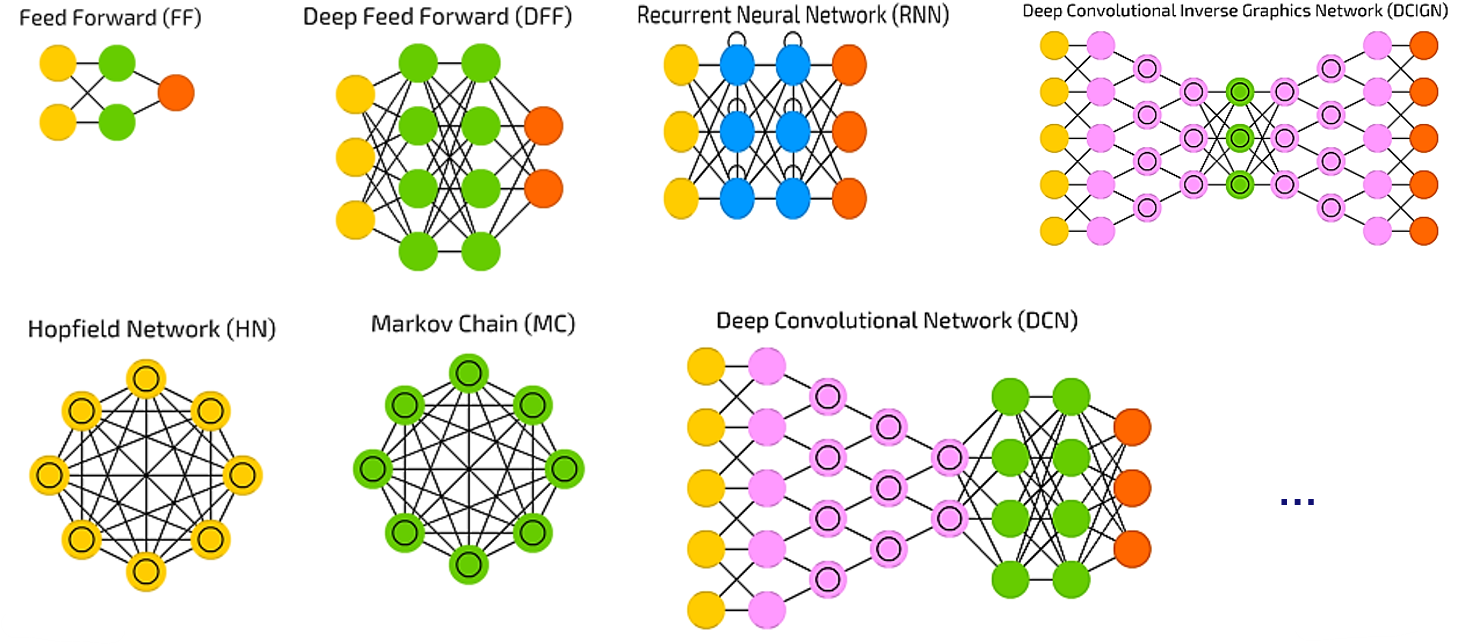
\includegraphics[width=0.9\textwidth]{assets/nn/fnn__types_topologies.png}
  \caption{Different types and topologies of NNs}
  \label{fig:6_fnn_types}
\end{figure}

One very often used architecture is the \textbf{convolutional NN}\sidenote{Convolutional Neural Network} (CNN) as shown in \ref{fig:6_fnn_cnn}. The intuitive idea is to have a hierarchy of visual elements that start by identifying edges using filters etc. and then move to more complex shapes. The extracted features then can be used for classification. CNNs are therefore best applied when the order of features matters, e.g. to successfully capture the spatial and temporal dependencies.

\begin{figure}[H]
  \centering
  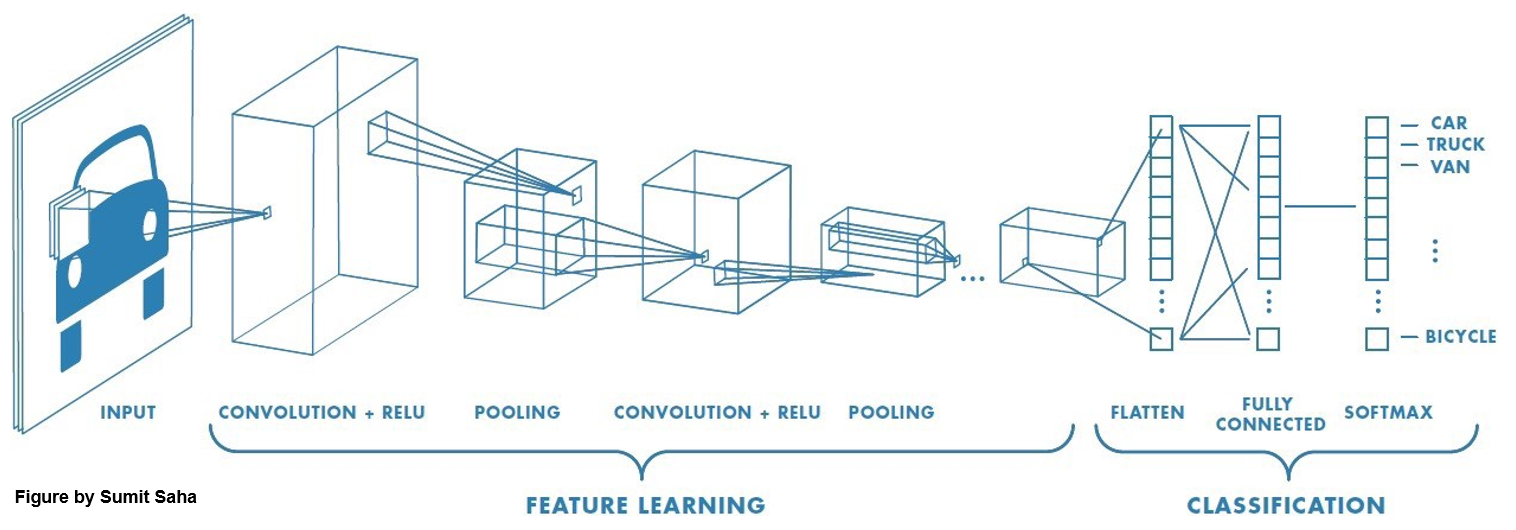
\includegraphics[width=0.8\textwidth]{assets/nn/fnn__cnn.png}
  \caption{CNN architecture}
  \label{fig:6_fnn_cnn}
\end{figure}

Another exemplary more complex architecture is the \textbf{recurrent NN}\sidenote{Recurrent Neural Network} (RNN), also known as Long Short-Term Memory (LSTM). This network processes sequences of data such as speech or video. It can find the next-following most-fitting element for a sequence. The details of this network architecture are not discussed here.
\begin{note}\begin{itemize}
  \item E.g.: "I lived in the Netherlands and speak perfectly \textcolor{burntorange}{Dutch}"
  \item E.g.: "2, 4, 16, 32, 64, \textcolor{burntorange}{128}"
\end{itemize}\end{note}

\begin{figure}[H]
  \centering
  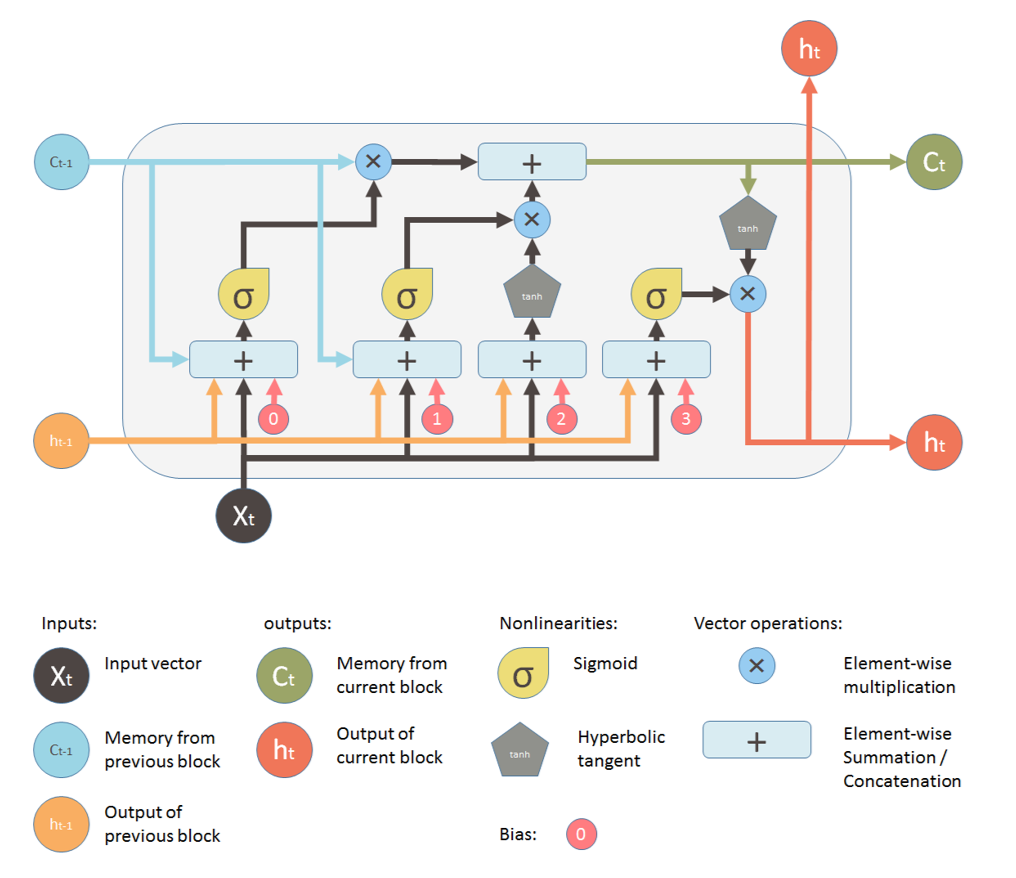
\includegraphics[width=0.55\textwidth]{assets/nn/fnn__rnn.png}
  \caption{RNN architecture}
  \label{fig:6_fnn_rnn}
\end{figure}

For this course, we're only gonna look at \textbf{feedforward neural networks}\sidenote{Feedforward Neural Networks} (FNN), also called multi-layer perceptrons, that don't contain any loops\footnote{Like in RNNs} or special layers\footnote{Like in CNNs}. This means we have:
\begin{itemize}
  \item Multiple simple perceptrons are arranged in a way that \textbf{layers} can be identified, and connections only exist to the next layer.
  \item The weights of the connection (in between two layers) can be changed or trained.
  \item The activation function (just as in a single-perceptron case) calculates whether the neuron fires or not.
\end{itemize}

To see, that FNNs really can express more functions than single-layer networks, we'll again consider the "XOR" example. As can be seen in \ref{fig:6_fnn_xor}. The result can be generalized, such that any boolean function with two input values can be represented by a two-layer perceptron.

\begin{figure}[H]
  \centering
  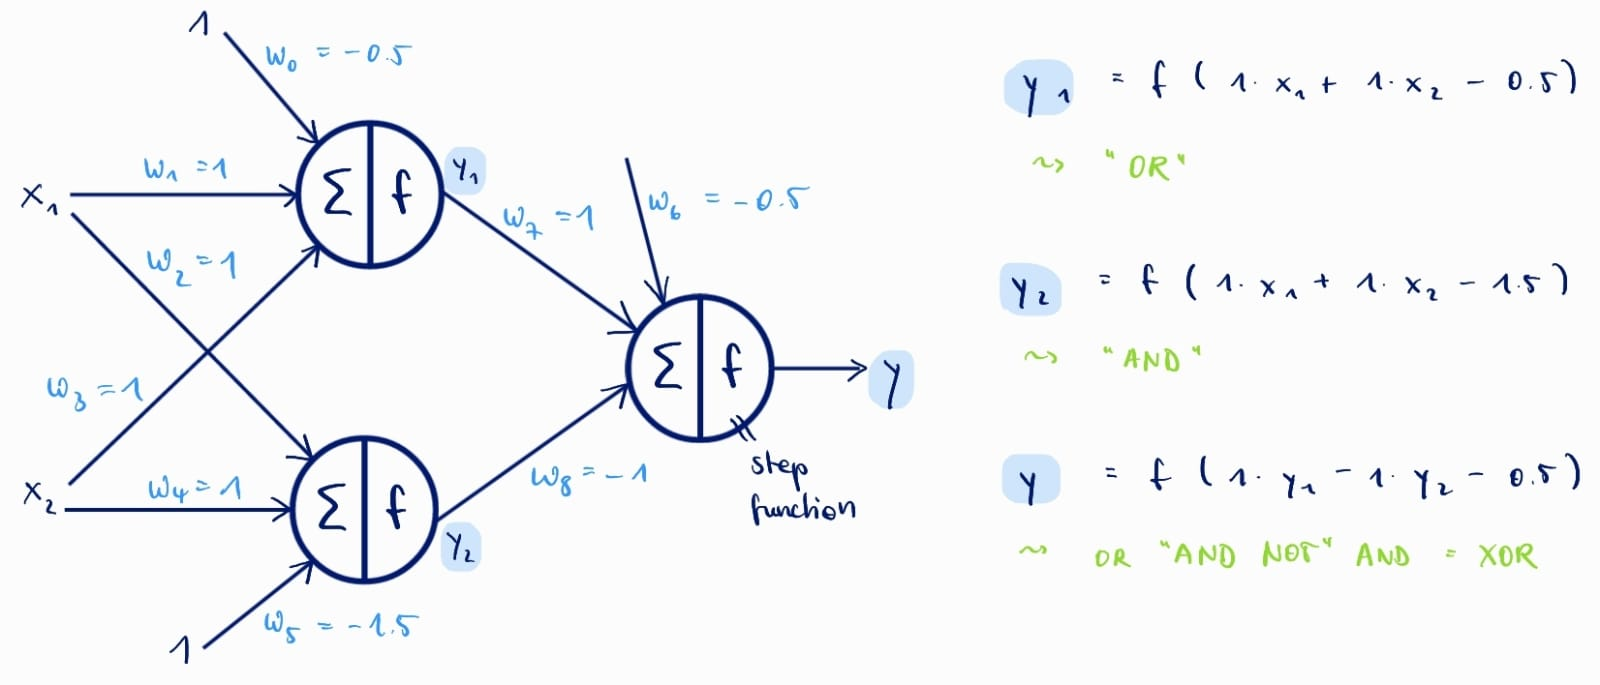
\includegraphics[width=0.9\textwidth]{assets/nn/fnn__xor.png}
  \caption{XOR with FNN}
  \label{fig:6_fnn_xor}
\end{figure}

To lead us through the whole chapter, we'll introduce a general 2-layer FNN implementing the function
\begin{align*}
  y_k(\cv{x}, \cv{w}) = f\left(\sum_{j=0}^M w_{jk}^{(2)}\cdot \underbrace{h\left(\sum_{i=0}^D w_{ij}^{(1)}x_i\right)}_{=:z_j}\right), \forall k\in[N]
\end{align*}
\begin{itemize}
  \item Weights are notated as $w_{\text{from to}}^{(\text{layer})}$.
  \item $f$ and $h$ represent activation functions (can be different, but every layer is assumed to have the same activation function on all its neurons).
  \item We have input dimension $D$, $M$ nodes in the hidden layer, and $N$ output neurons.
  \item The hidden units with their activation functions can express non-linear functions.
\end{itemize}

\begin{figure}[H]
  \centering
  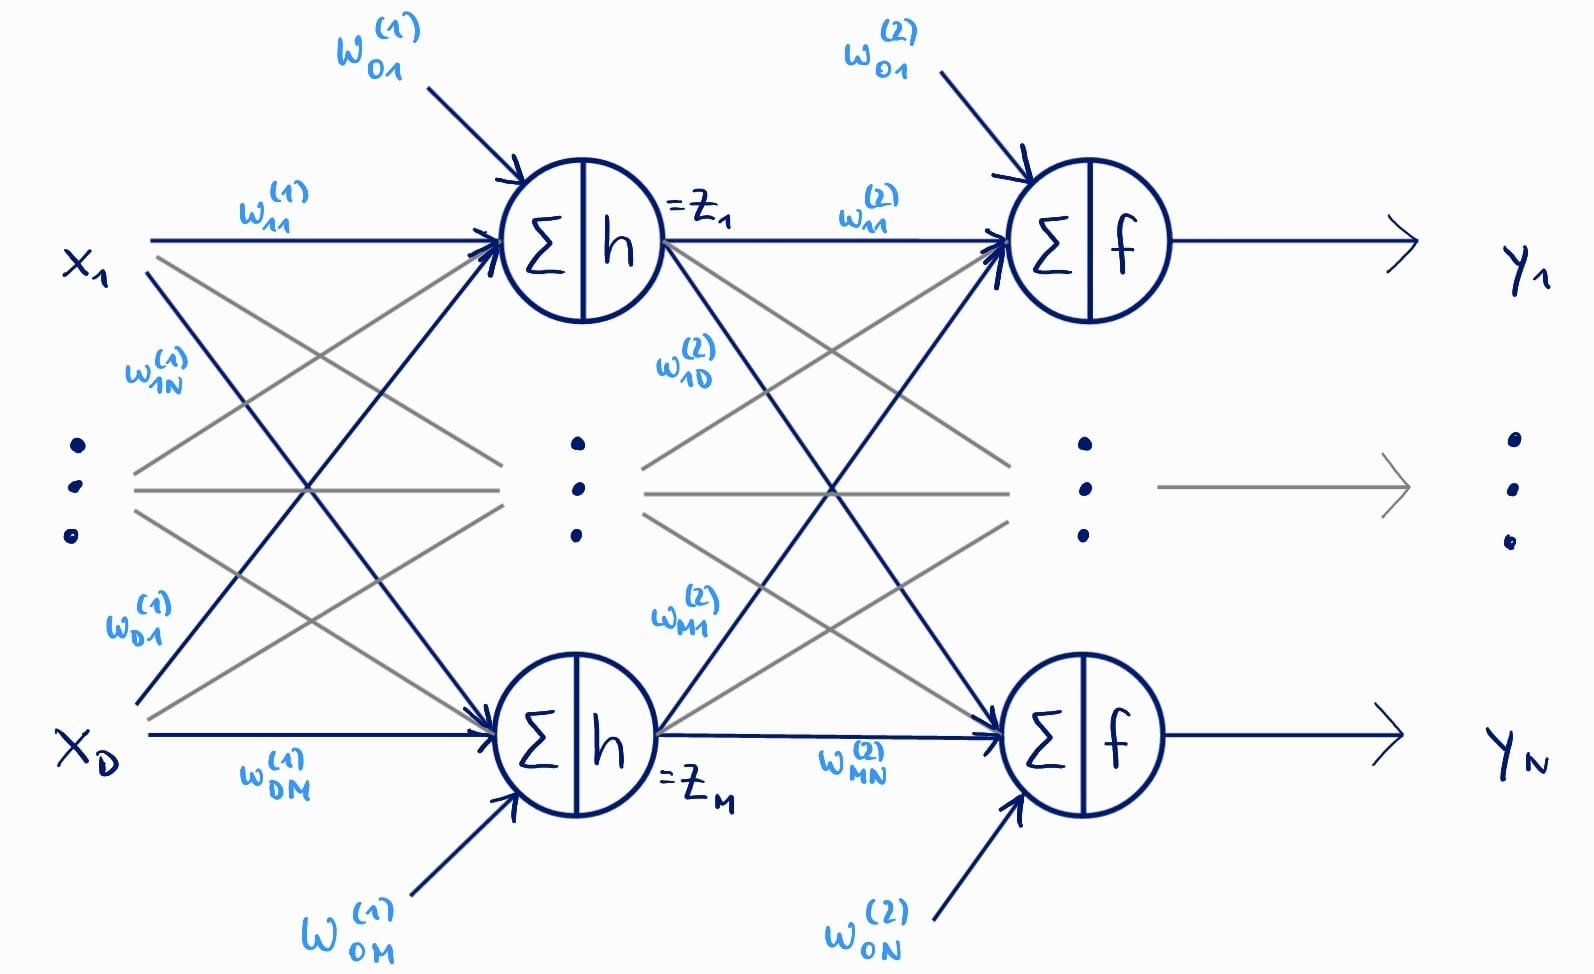
\includegraphics[width=0.7\textwidth]{assets/nn/fnn__architecture.png}
  \caption{2-layer FNN architecture}
  \label{fig:6_fnn_arch}
\end{figure}
